
\usepackage[utf8]{inputenc}
%\usepackage{ucs}
\usepackage{amsmath}
\usepackage{amsfonts}
\usepackage{amssymb}
\usepackage{multicol}
\usepackage{graphicx}
%\usepackage{hyperref}		% automatic included by beamer
\usepackage{tikz}
\usetikzlibrary{arrows,positioning,shapes}
\usepackage{listings}
\usepackage{multicol}
\usepackage{appendixnumberbeamer}
\usepackage{pstricks}
\usepackage{marvosym}
\usepackage{biblatex}

\newcommand{\code}[1]{\texttt{#1}}

\title{understanding the perf file format}
%\subtitle{}
\author{Urs F\"assler}
\date{01.09.2011}
\institute
{
  CERN Openlab
}
%\subject{}

%\bibliographystyle{plain}
\bibliography{../../report/literature}

\usetheme{Madrid}
\beamertemplatenavigationsymbolsempty

\tikzstyle{pointer}=[->,thick]
\tikzstyle{instance}=[->,thick,dashed]
\tikzstyle{connection}=[thick,dotted]
\tikzstyle{call}=[pointer]
\tikzstyle{use}=[instance]

\tikzstyle{struct}=[anchor=center,draw=black, minimum height=1 cm,top color=white, bottom color=yellow!30,thick, text centered,align=center]
\tikzstyle{entry}=[struct,rotate=90,minimum width=3 cm]
\tikzstyle{funcfile}=[struct,minimum width=3 cm]
\tikzstyle{edgelabel}=[text centered,align=center,fill opacity=.75,fill=white,text opacity=1]


\begin{document}
\begin{frame}[plain]
  \titlepage
\end{frame}

\setcounter{framenumber}{0}

\section{Problem}
\begin{frame}{Problem\only<handout>{ \cite{Jarp2010}}}
\begin{itemize}
  \item processors does not get faster
  \item more into parallel computing
  \item software has to be improved
\pause
  \item performance monitoring to find bottlenecks
  \item performance monitoring system of Linux is perf
  \item understanding monitoring system $\rightarrow$ extract relevant information
\end{itemize}
\end{frame}

\section{Process}
\begin{frame}{Process (1)}
\begin{itemize}
  \item sparse online resources
  \item perf report reads the data file
\pause
  \begin{itemize}
    \item stepping through code with debugger
    \item static analyze code
    \item analyzing data structures
\pause
    \item[$\Rightarrow$] Pitfall: overseen data structures
  \end{itemize}
\end{itemize}
\begin{center}
  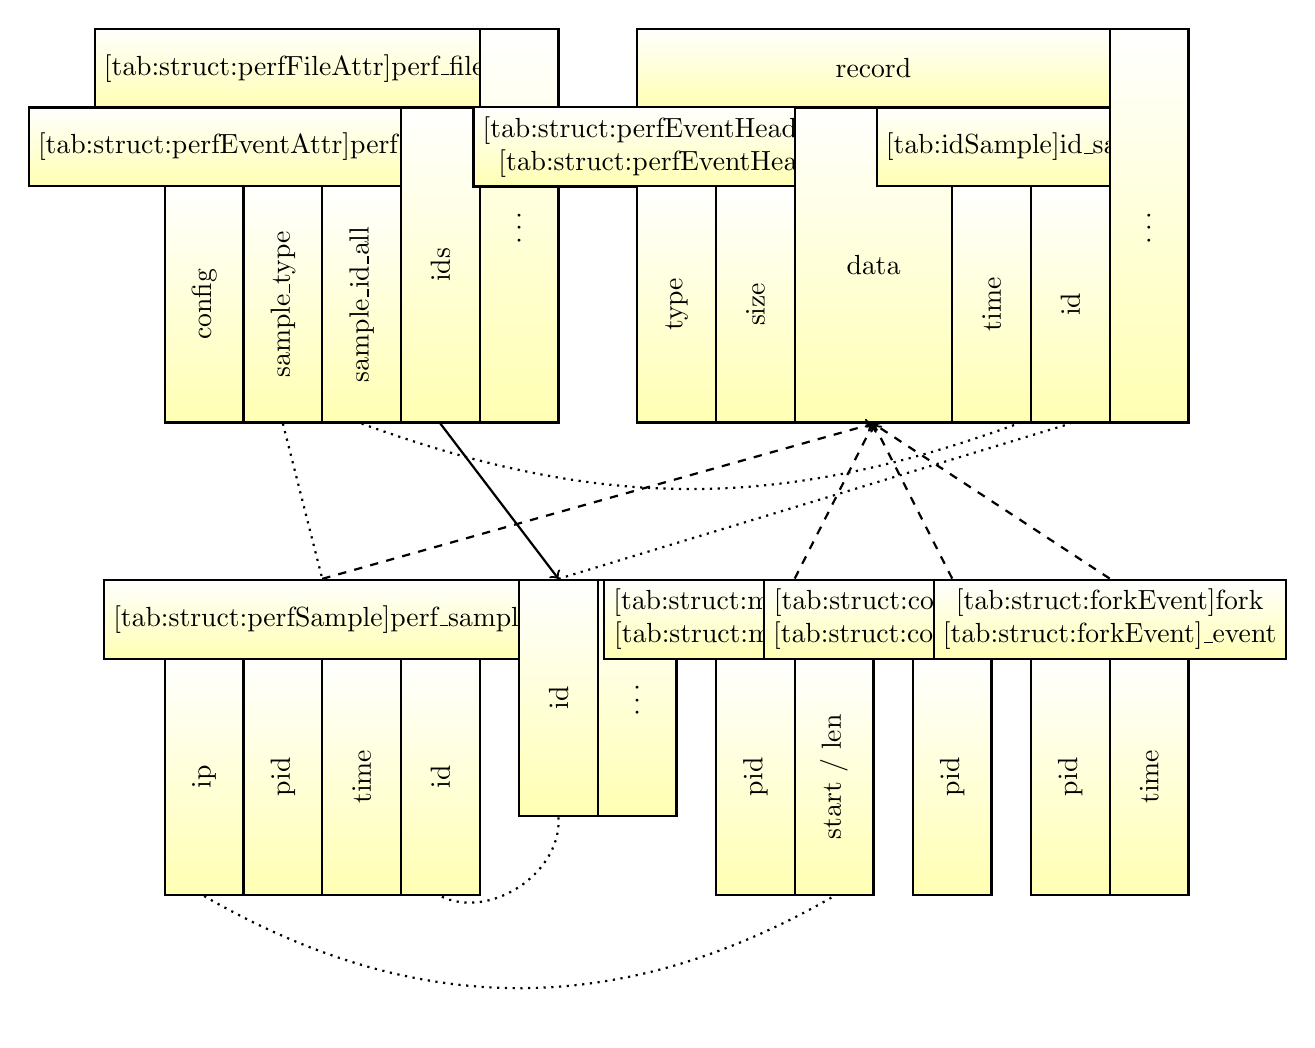
\begin{tikzpicture}[scale=1,transform shape]

\begin{scope}[xshift=0cm,yshift=-6cm]
  \node [struct,minimum width=4 cm] at (-0.5,0) (attrDecl){\hyperref[tab:struct:perfFileAttr]{perf\_file\_attr}};
  \node [struct,minimum width=3 cm] at (-1,-1) (){\hyperref[tab:struct:perfEventAttr]{perf\_event\_attr}};
  \node [entry] at (-2.0,-3) (config){config};
  \node [entry] at (-1.0,-3) (sampleType){sample\_type};
  \node [entry] at ( 0.0,-3) (idSampleBit){sample\_id\_all};
  \node [entry,minimum width=4 cm] at ( 1.0,-2.5) (ids){ids};
  \node [entry,minimum width=5 cm] at ( 2,-2) (){\ldots};
\end{scope}

\begin{scope}[xshift=7cm,yshift=-6cm]
  \node [struct,minimum width=6 cm] at (-0.5,0) (eventDecl){record};
  \node [struct,minimum width=2 cm] at (-2.5,-1) (){\hyperref[tab:struct:perfEventHeader]{perf\_event}\\\hyperref[tab:struct:perfEventHeader]{\_header}};
  \node [entry] at (-3,-3) (){type};
  \node [entry] at (-2,-3) (){size};
  \node [struct,minimum width=2 cm,minimum height=4 cm] at (-0.5,-2.5) (data){data};
  \node [struct,minimum width=2 cm] at (1.5,-1) (){\hyperref[tab:idSample]{id\_sample}};
  \node at (1.5,-4.5) (idSample) {};
  \node [entry] at ( 1,-3) (idSampleTime){time};
  \node [entry] at ( 2,-3) (idSampleId){id};
  \node [entry,minimum width=5 cm] at ( 3,-2) (){\ldots};
\end{scope}

\begin{scope}[xshift=-0.5cm,yshift=-13cm]
  \node [struct,minimum width=4 cm] at (0,0) (perfSample){\hyperref[tab:struct:perfSample]{perf\_sample}};
  \node [entry] at (-1.5,-2) (sampleIp){ip};
  \node [entry] at (-0.5,-2) (samplePid){pid};
  \node [entry] at ( 0.5,-2) (sampleTime){time};
  \node [entry] at ( 1.5,-2) (sampleId){id};
\end{scope}

\begin{scope}[xshift=3cm,yshift=-13cm]
  \node [entry] at (-0.5,-1) (idDecl){id};
  \node [entry] at ( 0.5,-1) (){\ldots};
\end{scope}

\begin{scope}[xshift=5.5cm,yshift=-13cm]
  \node [struct,minimum width=2 cm] at (0,0) (mmapEvent){\hyperref[tab:struct:mmapEvent]{mmap}\\\hyperref[tab:struct:mmapEvent]{\_event}};
  \node [entry] at (-0.5,-2) (mmapPid){pid};
  \node [entry] at ( 0.5,-2) (mmapRange){start / len};
\end{scope}

\begin{scope}[xshift=7.5cm,yshift=-13cm]
  \node [struct,minimum width=1 cm] at (0,0) (commEvent){\hyperref[tab:struct:commEvent]{comm}\\\hyperref[tab:struct:commEvent]{\_event}};
  \node [entry] at (0,-2) (commPid){pid};
\end{scope}

\begin{scope}[xshift=9.5cm,yshift=-13cm]
  \node [struct,minimum width=2 cm] at (0,0) (forkEvent){\hyperref[tab:struct:forkEvent]{fork}\\\hyperref[tab:struct:forkEvent]{\_event}};
  \node [entry] at (-0.5,-2) (forkPid){pid};
  \node [entry] at ( 0.5,-2) (forkTime){time};
\end{scope}


\path [pointer] (ids.west) edge (idDecl.east);
\path [connection,bend right=20] (idSampleBit.west) edge (idSample.west);
\path [connection,bend left=60] (idDecl.west) edge (sampleId.west);
\path [connection] (idDecl.east) edge (idSampleId.west);
\path [connection] (sampleType.west) edge (perfSample.north);
\path [connection,bend right=30] (sampleIp.west) edge (mmapRange.west);
\path [instance] (perfSample.north) edge (data.south);
\path [instance] (commEvent.north) edge (data.south);
\path [instance] (mmapEvent.north) edge (data.south);
\path [instance] (forkEvent.north) edge (data.south);


\end{tikzpicture}

\end{center}
\end{frame}

\begin{frame}{Process (2)}
\begin{itemize}
  \item analyzing code / structures $\rightarrow$ thinking $\rightarrow$ idea $\rightarrow$ verifying
  \begin{itemize}
    \item write code to see if it works
    \item compare it with perf report
  \end{itemize}
\pause
  \item Andrzej /$\rightarrow$ contact to other people
\end{itemize}
\end{frame}

\section{Achievements}
\begin{frame}{Achievements}
\begin{itemize}
  \item good understanding of perf data format
\pause
  \item ''proof of concept'' application (readperf), verified against perf report
  \begin{itemize}
    \item only 1k lines of code (perf 34k)
    \item no kernel code / dependencies
    \item small dependencies
  \end{itemize}
\pause
  \item report\only<handout>{\cite{Faessler2011}} as description of file format and readperf
\pause
  \item[$\Rightarrow$] basis for performance analysis
\end{itemize}
\end{frame}

\section{Conclusion}
\begin{frame}{Conclusion}
\begin{itemize}
  \item perf seems like historically grown
  \begin{itemize}
    \item[$\Rightarrow$] complex, difficult to understand
  \end{itemize}
\pause
  \item good solution for analyzing software
  \begin{itemize}
    \item perf tools
    \item kernel interface
  \end{itemize}
\pause
  \item Open Source is good, still need time to understand the code
  \begin{itemize}
    \item[$\Rightarrow$] but without code it would be much harder
  \end{itemize}
\end{itemize}
\end{frame}


\only<handout>{
  \appendix
\section{Appendix}

\begin{frame}{Analyze virtualized machine}
\code{perf} has support for the Kernel-based Virtual Machine (KVM \cite{kvm}). For the performance measurement, an argument tells \code{perf} that the machine using KVM should be monitored. It uses the PMU of the host. It seems that also detailed information is available if the host machine has access to the guests \code{/proc/} files. Measures of hardware counters from inside the virtual machine is not supported.

VirtualBox \cite{virtualbox} is not supported. This has two consequences. First, \code{perf} on the host can not record data about the guest. Second, there is no PMU in the virtual machine and therefore \code{perf} can not record hardware counters.
\end{frame}

\only<handout>{
\begin{frame}{literature}
\begin{scriptsize}
  \printbibliography
\end{scriptsize}
\end{frame}
}

}

\end{document}
